\chapter{Aufgabe 3}
\textit{Überprüfen Sie,  welche  ihrer  manuell  durch geführten  Optimierungen durch  den Einsatz  geeigneter  Compiler-Flags  bzw.  Optimierungsstufen  auch  vom  Compiler realisiert werden.} \newline

Als Compiler Flags haben wir $-O1$, $-O2$ und $-O3$ ausprobiert. Zuerst betrachten wir den gcc Compiler. Die Ausführzeiten für den gcc Compiler sind in den Abbildungen \ref{gccO1}, \ref{gccO2} und \ref{gccO3} gezeigt. Die GFLOP/s sind in den Abbildungen \ref{GgccO1}, \ref{GgccO2} und \ref{GgccO3} zusammengefasst. Der mittels $-O1$ compilierte Quelltext ist im Vergleich zum $-O0$ compilierten Quelltext deutlich schneller. Die geringste Steigerung gibt es für den originalen Quelltext. Hier wird die Matrix nur rund 40\% schneller ausgeführt. Die Steigerung, falls die $B$ Matrix vorher transponiert wurde, beträgt ungefähr 325\%. Das Ausrollen des Quelltextes ist 90\% schneller, falls es mit $-O1$ compiliert wird. Das Tiling benötigt ungefähr halb soviel Zeit. 
Die Ausführzeiten zwischen $-O1$, $-O2$ und $-O3$ compilierten Quelltext sind identisch.

Die Zeiten für den Intel Compiler sind in den Abbildungen \ref{iccO1}, \ref{iccO2} und \ref{iccO3} aufgeführt. Die GFLOP/s Performance ist in den Abbildungen \ref{GiccO1}, \ref{GiccO2} und \ref{GiccO3} zusammengefasst. Auf der $-O1$ Stufe ist der Intel Compiler mit dem gcc Compiler vergleichbar. Die Multiplikation und die Transponierung der $B$ Matrix sind gleich schnell. Ein zusätzliches ausrollen der inneren Schleife wird von gcc Compiler besser übersetzt. Der gcc erzeugt rund 15\% schnelleren Code. Bei der Matrixmultiplikation mit Tiling ist der gcc 0.5 GFLOP/s schneller. Das $-O2$ Flag erzeugt einen deutlichen Performancegewinn beim Intel Compiler. Am deutlichsten wird dies am Quelltext der unverändert compiliert wird. Dieser wird 15x schneller ausgeführt, als mit $-O1$ Flag, und erreicht 4.68 GFLOP/s. Die Transponierung der $B$ Matrix ist mit $-O2$ Flag die schnellste Multiplikationsvariante. Diese Variante wird 2,5 mal schneller ausgeführt als mit $-O1$ Flag. Die Unroll variante ist ungefähr doppelt so schnell. Sie ist aber 1,6 GFLOP/s langsamer als die Transpositionierungs Variante. Bei der Blocking Multiplikation gibt es keine Änderung. Zwischen den $-O2$ und $-O3$ compilierten Varianten gibt es nur für die Ausrollung Variante einen Unterschied. Die Ausrollung ist mit $-O3$ Flag, 1,6 GFLOP/s langsamer als die mit $O2$ compilierten. 

Das $-O1$ Flag des gcc Compiler aktiviert eine Vielzahl von Optimierungen. Beispiels weiße versucht $-fforward-propagate$ zwei Anweisungen zu kombinieren und zu vereinfachen. Das Flag $-freorder-blocks$ vertauscht Basisblöcke um die Codelokalität zu erhöhen. Das $-O2$ und das $-O3$ Flag erhöhen die Performance nicht. 
Der Größe unterschied zwischen den Intel Compiler und den gcc Compiler ist die $-O2$ Optimierungsstufe. Auf der Intel Homepage \footnote{\url{https://software.intel.com/en-us/articles/step-by-step-optimizing-with-intel-c-compiler}} steht: 

``This option enables optimizations for speed. This is the generally recommended optimization level. The compiler vectorization is enabled at O2 and higher levels. With this option, the compiler performs some basic loop optimizations, inlining of intrinsic, Intra-file interprocedural optimization, and most common compiler optimization technologies.''

\begin{table}[h]
  \begin{tabular}{l|l|l|l|l|l|l}
  & \multicolumn{3}{c|}{gcc} &                                      \multicolumn{3}{|c}{Intel} \\

                          & -O1    & -O2    & -O3    &  -O1   & -O2    & -O3 \\
                            \hline
  Keine Optimierung       & 6.5820 & 6.5765 & 6.5713 & 6.7796 & 0.4591 & 0.4527\\
  Transponierung          & 0.8771 & 0.8773 & 0.8827 & 0.8768 & 0.3622 & 0.3617\\
  Transponierung + Unroll & 0.7882 & 0.7885 & 0.7764 & 0.8717 & 0.4965 & 0.7891\\
  Blocking Blockgröße 32  & 0.8339 & 0.8369 & 0.8435 & 1.0509 & 1.0386 & 1.0414\\


  \hline
 \end{tabular}
 \caption{Zusammenfassung der Ausführzeiten für eine Multiplikation von zwei Matrizen der Größe 1024. Die Zeiten sind in Sekunden.}
\end{table}

\begin{table}[h]
  \begin{tabular}{l|l|l|l|l|l|l}
  & \multicolumn{3}{c|}{gcc} &                                      \multicolumn{3}{|c}{Intel} \\

                          & -O1    & -O2    & -O3    &  -O1   & -O2    & -O3 \\
                            \hline
  Keine Optimierung       & 0.33   & 0.33   & 0.33   &  0.29  & 4.68   & 4.74 \\
  Transponierung          & 2.45   & 2.45   & 2.43   &  2.34  & 5.93   & 5.94 \\
  Transponierung + Unroll & 2.72   & 2.72   & 2.77   &  2.43  & 4.33   & 2.72 \\
  Blocking Blockgröße 32  & 2.58   & 2.57   & 2.55   &  2.72  & 2.07   & 2.06 \\

  \hline
 \end{tabular}
  \caption{Zusammenfassung der GFLOP/s für eine Multiplikation von zwei Matrizen der Größe 1024.}
\end{table}

\begin{figure}[h]
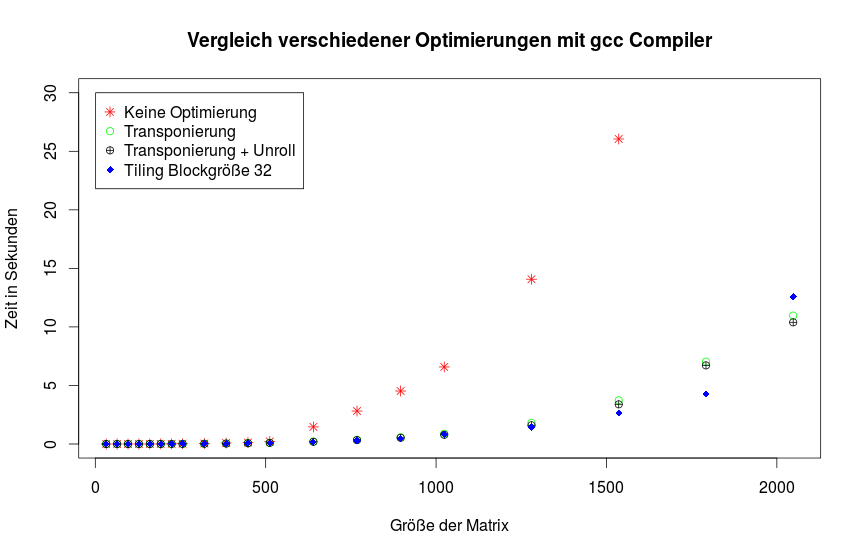
\includegraphics[scale = 0.45]{Bilder/gccO1.png}
\caption{Vergleich der Laufzeiten verschiedener Optimierungen mit dem gcc Compiler. Der Quelltext wurde mit den Parametern -O1 -std=c99 compiliert.}
\noindent\rule{14cm}{0.4pt}
\label{gccO1}
\end{figure}

\begin{figure}[h]
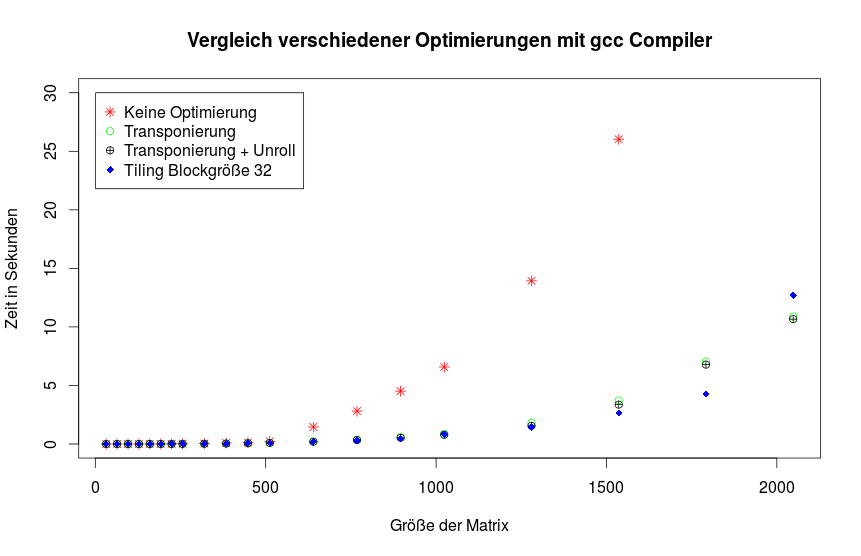
\includegraphics[scale = 0.45]{Bilder/gccO2.png}
\caption{Vergleich der Laufzeiten verschiedener Optimierungen mit dem gcc Compiler. Der Quelltext wurde mit den Parametern -O2 -std=c99 compiliert.}
\noindent\rule{14cm}{0.4pt}
\label{gccO2}
\end{figure}

\begin{figure}[h]
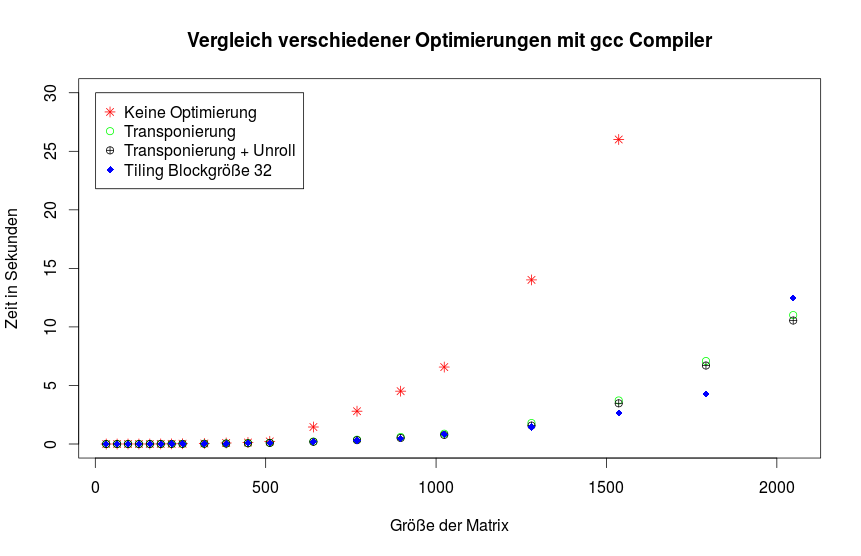
\includegraphics[scale = 0.45]{Bilder/gccO3.png}
\caption{Vergleich der Laufzeiten verschiedener Optimierungen mit dem gcc Compiler. Der Quelltext wurde mit den Parametern -O3 -std=c99 compiliert.}
\noindent\rule{14cm}{0.4pt}
\label{gccO3}
\end{figure}

\begin{figure}[h]
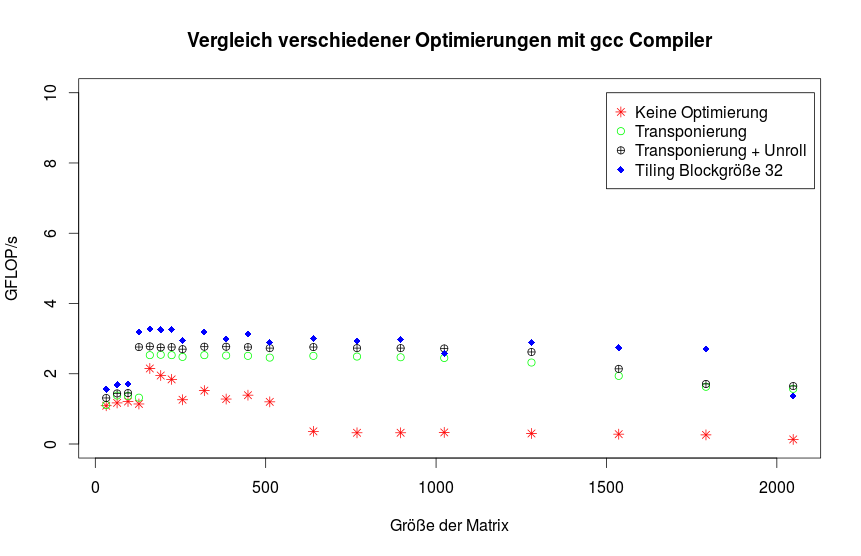
\includegraphics[scale = 0.45]{Bilder/GgccO1.png}
\caption{Vergleich der GFLOP/s verschiedener Optimierungen mit dem gcc Compiler. Der Quelltext wurde mit den Parametern -O1 -std=c99 compiliert.}
\noindent\rule{14cm}{0.4pt}
\label{GgccO1}
\end{figure}

\begin{figure}[h]
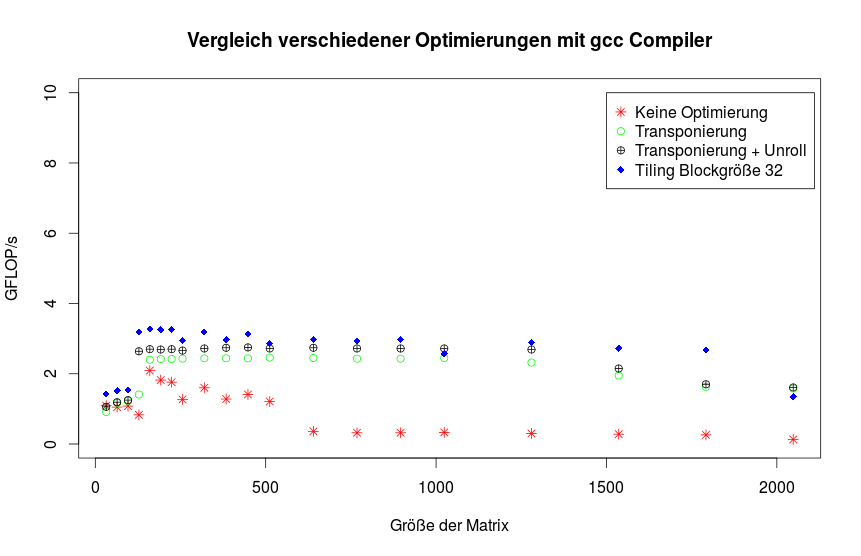
\includegraphics[scale = 0.45]{Bilder/GgccO2.png}
\caption{Vergleich der GFLOP/s verschiedener Optimierungen mit dem gcc Compiler. Der Quelltext wurde mit den Parametern -O2 -std=c99 compiliert.}
\noindent\rule{14cm}{0.4pt}
\label{GgccO2}
\end{figure}

\begin{figure}[h]
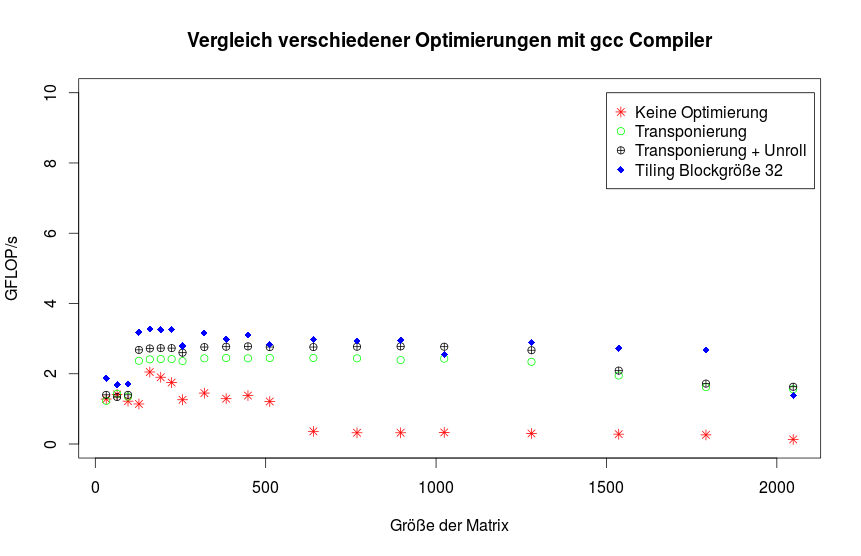
\includegraphics[scale = 0.45]{Bilder/GgccO3.png}
\caption{Vergleich der GFLOP/s verschiedener Optimierungen mit dem gcc Compiler. Der Quelltext wurde mit den Parametern -O3 -std=c99 compiliert.}
\noindent\rule{14cm}{0.4pt}
\label{GgccO3}
\end{figure}

\begin{figure}[h]
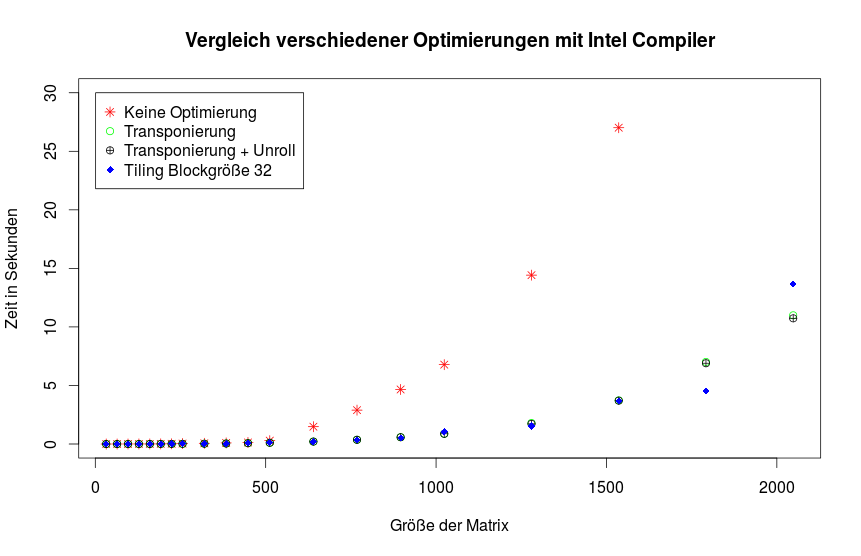
\includegraphics[scale = 0.45]{Bilder/iccO1.png}
\caption{Vergleich der Laufzeiten verschiedener Optimierungen mit dem Intel Compiler. Der Quelltext wurde mit den Parametern -O1 -std=c99 compiliert.}
\noindent\rule{14cm}{0.4pt}
\label{iccO1}
\end{figure}

\begin{figure}[h]
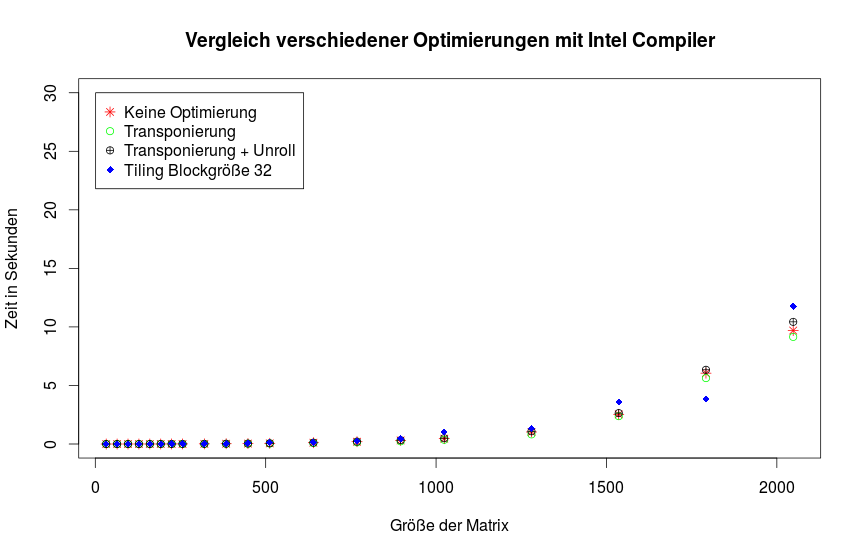
\includegraphics[scale = 0.45]{Bilder/iccO2.png}
\caption{Vergleich der Laufzeiten verschiedener Optimierungen mit dem Intel Compiler. Der Quelltext wurde mit den Parametern -O2 -std=c99 compiliert.}
\noindent\rule{14cm}{0.4pt}
\label{iccO2}
\end{figure}

\begin{figure}[h]
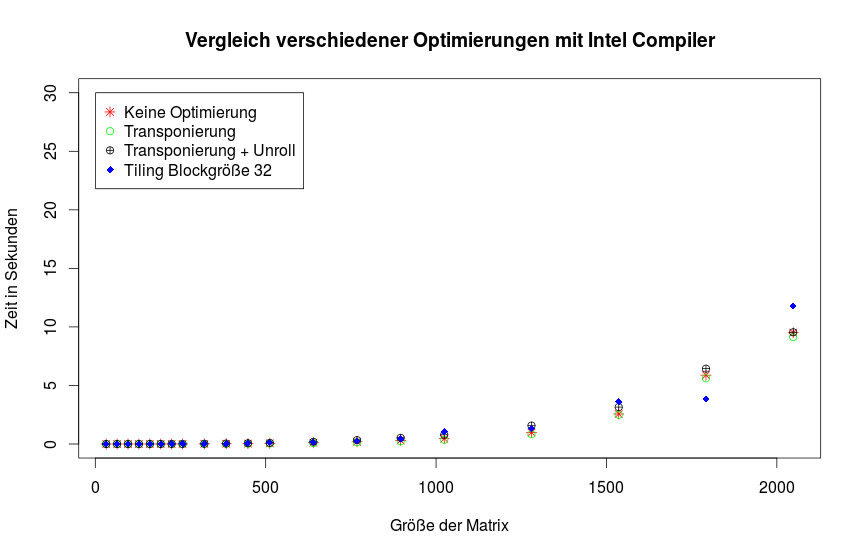
\includegraphics[scale = 0.45]{Bilder/iccO3.png}
\caption{Vergleich der Laufzeiten verschiedener Optimierungen mit dem Intel Compiler. Der Quelltext wurde mit den Parametern -O3 -std=c99 compiliert.}
\noindent\rule{14cm}{0.4pt}
\label{iccO3}
\end{figure}

\begin{figure}[h]
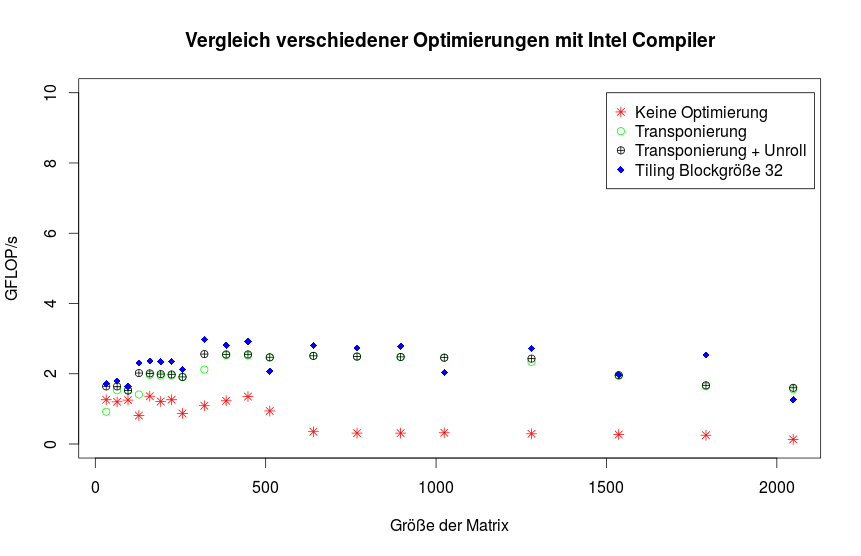
\includegraphics[scale = 0.45]{Bilder/GiccO1.png}
\caption{Vergleich der GFLOP/s verschiedener Optimierungen mit dem Intel Compiler. Der Quelltext wurde mit den Parametern -O1 -std=c99 compiliert.}
\noindent\rule{14cm}{0.4pt}
\label{GiccO1}
\end{figure}

\begin{figure}[h]
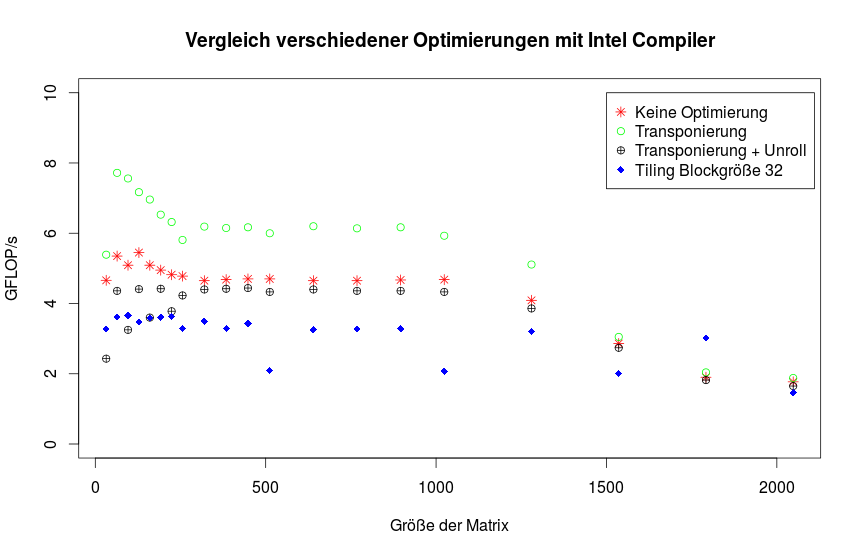
\includegraphics[scale = 0.45]{Bilder/GiccO2.png}
\caption{Vergleich der GFLOP/s verschiedener Optimierungen mit dem Intel Compiler. Der Quelltext wurde mit den Parametern -O2 -std=c99 compiliert.}
\noindent\rule{14cm}{0.4pt}
\label{GiccO2}
\end{figure}

\begin{figure}[h]
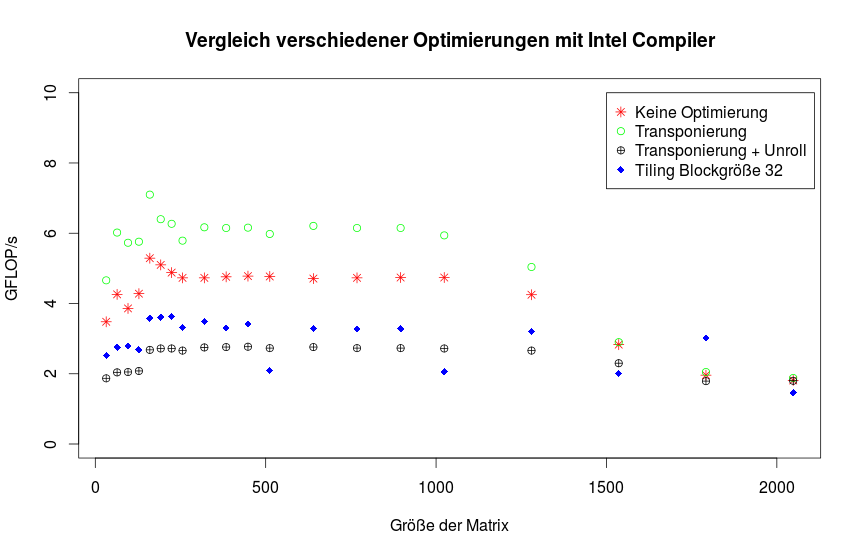
\includegraphics[scale = 0.45]{Bilder/GiccO3.png}
\caption{Vergleich der GFLOP/s verschiedener Optimierungen mit dem Intel Compiler. Der Quelltext wurde mit den Parametern -O3 -std=c99 compiliert.}
\noindent\rule{14cm}{0.4pt}
\label{GiccO3}
\end{figure}